
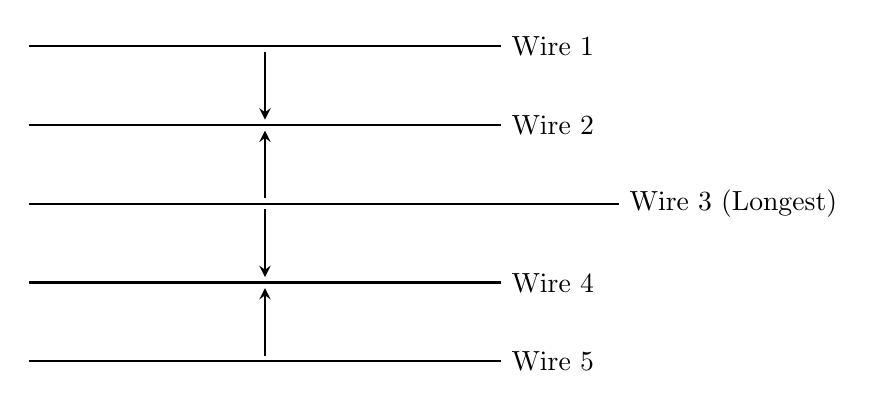
\begin{tikzpicture}[
    line/.style={thick},
    arrow/.style={->, thick, >=stealth, shorten <=2pt, shorten >=2pt}
]

    % Define the standard length and the extended length for the central line
    \def\standardL{6}
    \def\extendedL{7.5}
    \def\arrowX{3} % X-coordinate for where the arrows are placed

    % Horizontal lines (from top to bottom)
    \draw[line] (0, 4) -- (\standardL, 4) node[right] {Wire 1};
    \draw[line] (0, 3) -- (\standardL, 3) node[right] {Wire 2};
    \draw[line] (0, 2) -- (\extendedL, 2) node[right] {Wire 3 (Longest)};
    \draw[line] (0, 1) -- (\standardL, 1) node[right] {Wire 4};
    \draw[line] (0, 0) -- (\standardL, 0) node[right] {Wire 5};

    % Alternating arrows between the lines
    % Between Line 1 and 2: Pointing downwards
    \draw[arrow] (\arrowX, 4) -- (\arrowX, 3);
    
    % Between Line 2 and 3: Pointing upwards
    \draw[arrow] (\arrowX, 2) -- (\arrowX, 3);
    
    % Between Line 3 and 4: Pointing downwards
    \draw[arrow] (\arrowX, 2) -- (\arrowX, 1);
    
    % Between Line 4 and 5: Pointing upwards
    \draw[arrow] (\arrowX, 0) -- (\arrowX, 1);

\end{tikzpicture}

